%!TEX root = root.tex

\chapter{Benchmarking cancer driver gene predictions}
\label{chap:ch4}
\chaptermark{Cancer driver gene benchmark}

Rigorous and unbiased evaluation is necessary to inform users about the comparative utility of prediction methods. In many investigative domains, there is a generally accepted gold standard against which predictions can be benchmarked \cite{RN102, RN103}. However, only a limited number of genes have been fully vetted as cancer drivers. In previous work, driver prediction has been benchmarked by significant overlap with the Cancer Gene Census (CGC) \cite{RN91}, which is a manually curated list of likely but not necessarily validated driver genes \cite{RN54, RN53} or by agreement with a consensus gene list of drivers predicted by multiple methods \cite{RN96}. To our knowledge, a systematic framework for the evaluation of somatic mutations that can be generally applied has not been previously developed. Eight methods were evaluated: MutsigCV \cite{RN13}, ActiveDriver \cite{RN98}, MuSiC \cite{RN43}, OncodriveClust \cite{RN54}, OncodriveFM \cite{RN53}, OncodriveFML \cite{RN86}, Tumor Suppressor and Oncogenes (TUSON) \cite{RN71}, and 20/20+ \cite{RN70}. 

In this chapter, I present a framework for such evaluations. The framework has five components, some of which have been previously applied in isolation, but not as part of a unified system. I considered overlap with CGC, agreement between methods, comparison of observed vs. theoretical P values, number of significant genes predicted, and prediction consistency on independent partitions of the dataset. To implement this framework, I first collected 729,205 published somatic mutations from 34 cancer types \cite{RN14, RN71} \autoref{fig:benchmark_data}. These mutations were composed of single base substitutions and in-frame and out-of-frame insertions and deletions (indels) of less than 10 bp. I then compared various methods on the full pancancer set.

\begin{figure}
  \centering
  \makeatletter
  \let\@currsize\normalsize
  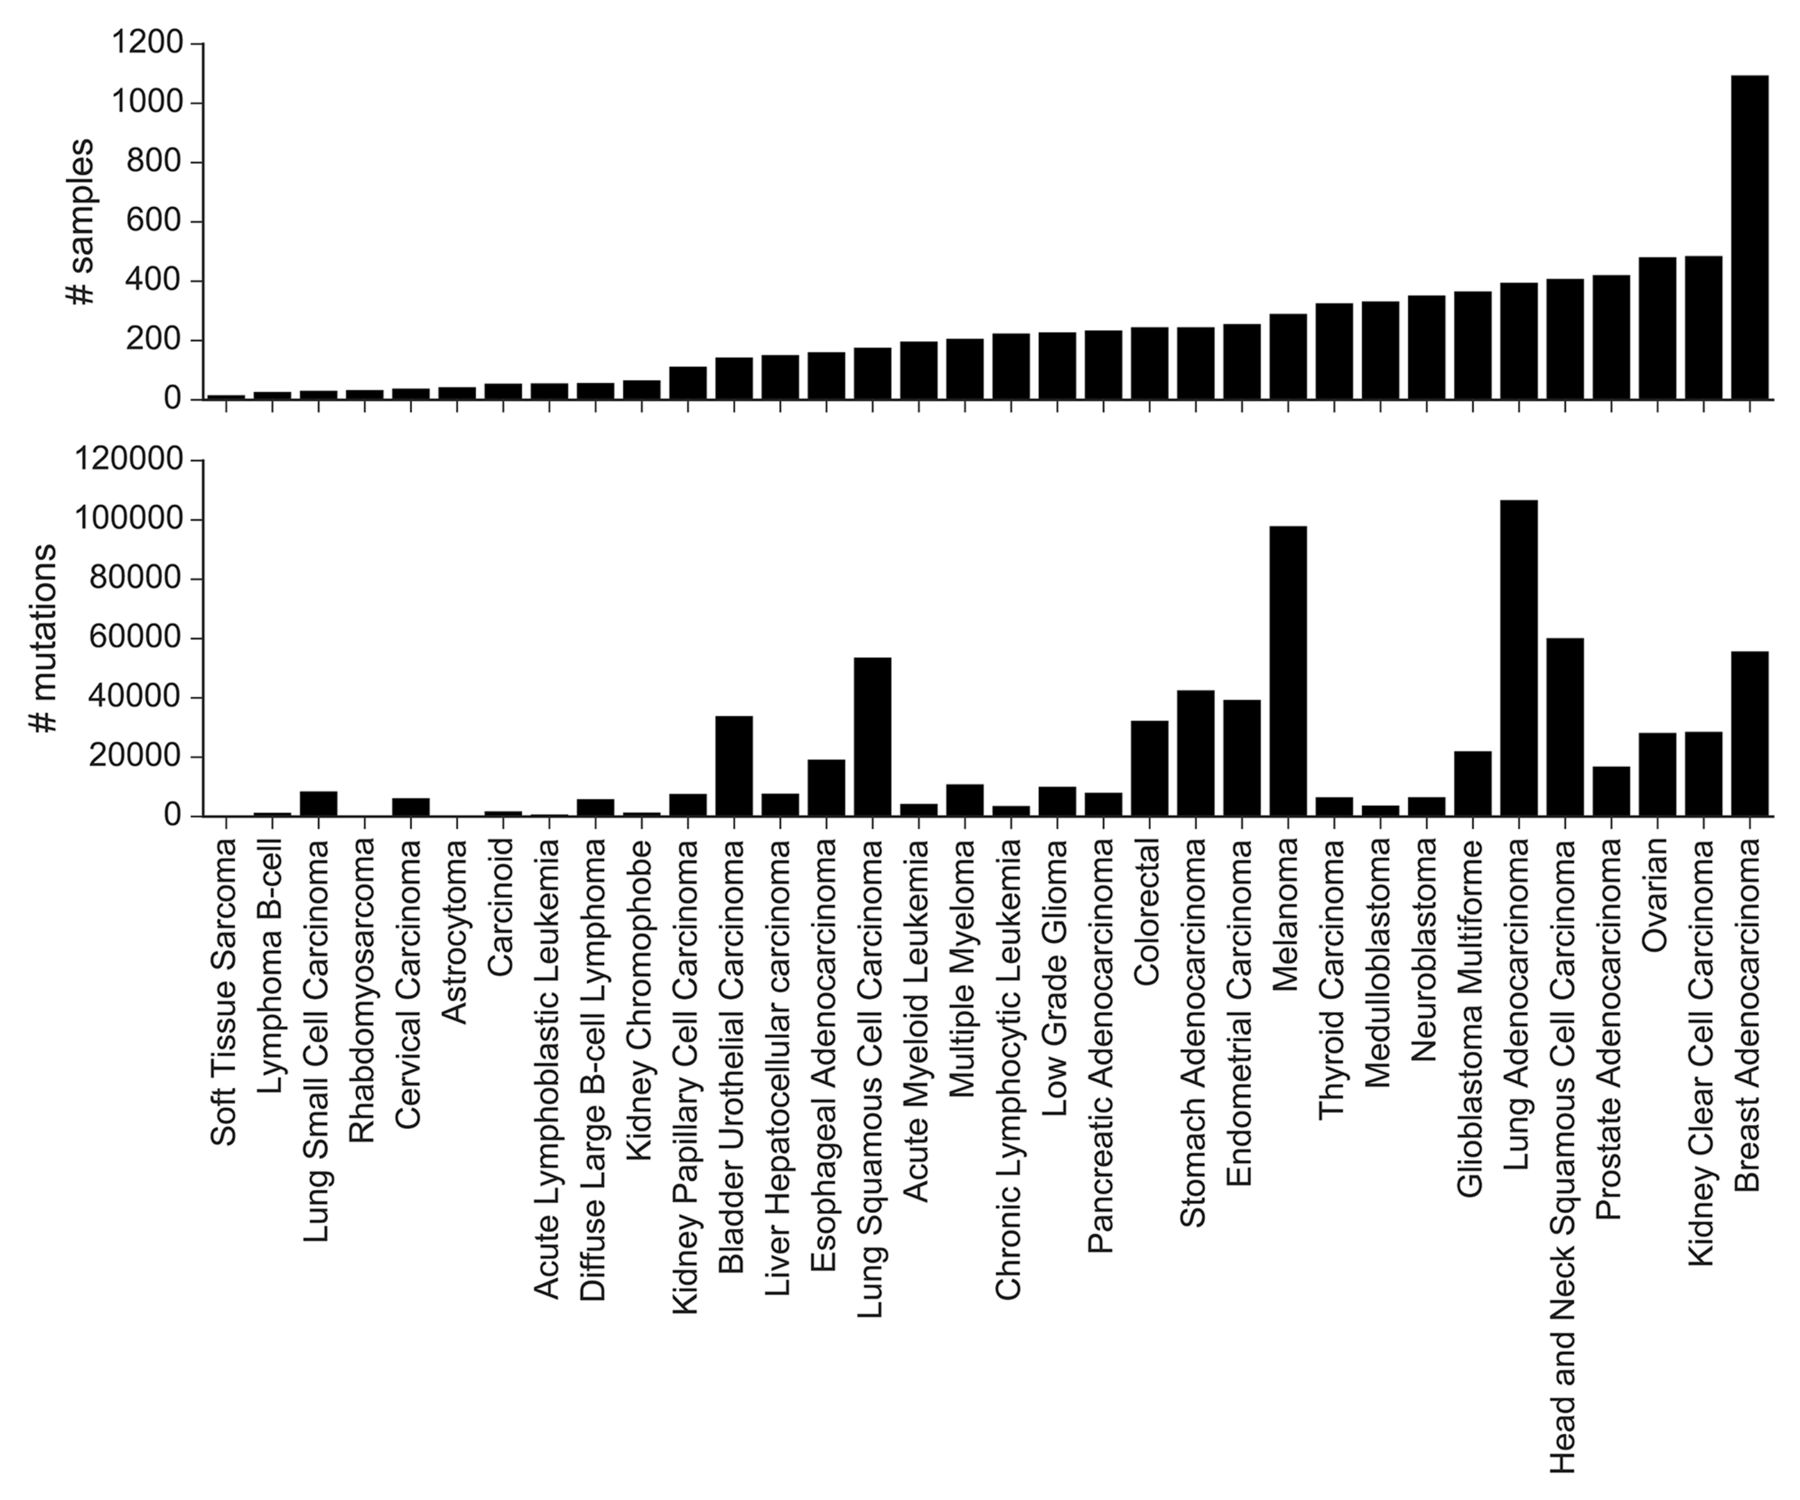
\includegraphics[width=0.9\linewidth]{figures/chapter4/study_size.jpg}
  \caption[Summary of evaluation dataset.]{Summary of evaluation dataset. The evaluation dataset consisted of mutations spanning 34 cancer types. All included mutations were small somatic variants. Cancer types are ordered from Left to Right by number of samples, ranging from 15 for soft-tissue sarcoma to 1,093 for breast adenocarcinoma, with an average of 232 samples per cancer type. These cancer types span a wide range of solid and several liquid cancers, including multiple tissues and cell types of origin, different background mutation rates, and different numbers of available samples. For each cancer type, total mutations and number of available samples are shown.}
  \label{fig:benchmark_data}
\end{figure}

\section{Overlap of the Driver Genes Predicted by Each Method}

First, I assessed overlap of the predicted driver genes with the CGC. I considered only those CGC genes typed as somatic, missense, frameshift, nonsense or splice site, excluding translocations, large amplifications/deletions, and other mutation consequence types not addressed in our study, yielding a total of 188 CGC genes. Although the driver genes predicted by all methods were enriched for CGC genes, the predicted drivers by any individual method did not contain a majority of CGC genes (\autoref{fig:benchmark_result}A). Three methods (20/20+, MutsigCV, and TUSON) had substantially higher fractions of predicted drivers in the CGC than the other methods. When I considered a subset of 99 CGC genes supported by functional studies \cite{RN99}, the results were very similar. The ranking of methods by fraction predicted was essentially the same as with the full CGC, with the three methods listed above having substantially higher fractions than the rest.

Genes predicted by more than one method may be more likely to be drivers \cite{RN96}. For each method, I calculated the fraction of predicted drivers that were unique or predicted by at least one, two, or three other methods (\autoref{fig:benchmark_method_overlap}). As shown in \autoref{fig:benchmark_method_overlap}, there was little consensus in prediction of driver genes among the methods. The majority (59-80\%) of genes identified by MuSiC, ActiveDriver, OncodriveClust, OncodriveFML, or OncodriveFM were not observed by any of the other seven methods. The fractions of genes identified by TUSON, 20/20+, and MutsigCV that were not identified as driver genes in at least one of the other seven methods was 14\%, 19\%, and 33\%, respectively. Although it is likely that some of the uniquely predicted drivers are bona fide, I could not find convincing literature support for the top-ranked unique predictions of MuSiC, ActiveDriver, and the Oncodrive methods. 

\begin{figure}
  \centering
  \makeatletter
  \let\@currsize\normalsize
  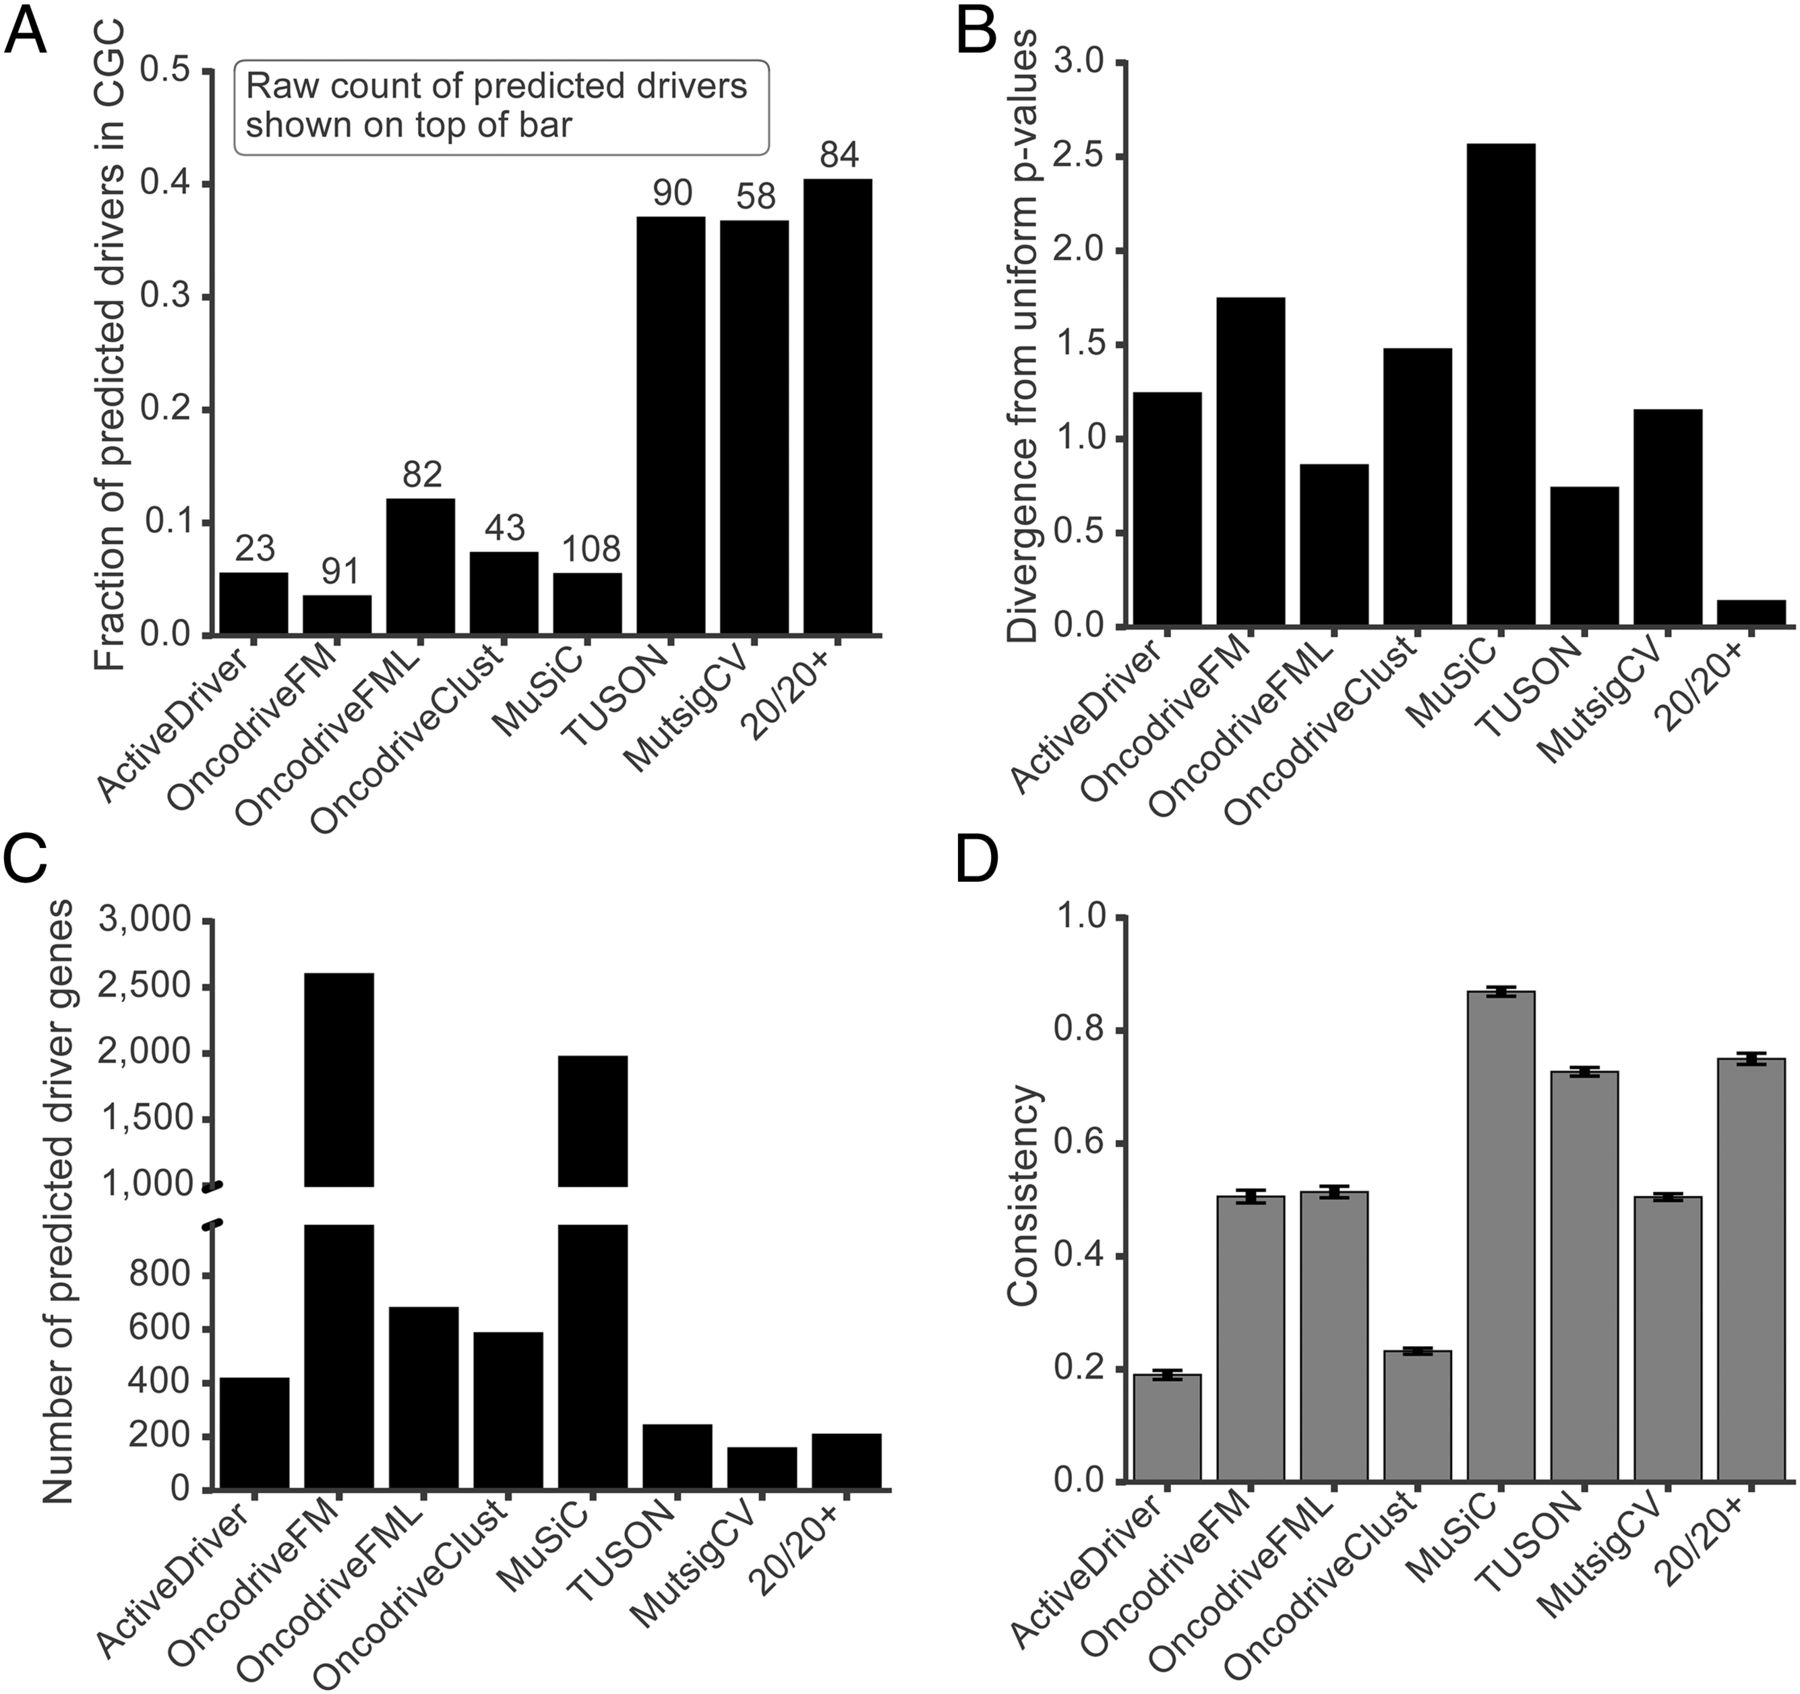
\includegraphics[width=0.9\linewidth]{figures/chapter4/evaluation.jpg}
  \caption[Outputs of eight driver prediction methods run through the evaluation protocol.]{Outputs of eight driver prediction methods run through the evaluation protocol. (A) Fraction of predicted driver genes (q ≤ 0.1) that are found in the Cancer Gene Census (CGC) (downloaded April 1, 2016). Raw count of predicted driver genes indicated on Top of each bar. (B) Divergence from uniform P values, measured as mean log fold change (MLFC) between a method's observed and desired theoretical P values. (C) Number of predicted driver genes. Driver gene is defined as having Benjamini-Hochberg adjusted P value, $q \leq 0.1$. (D) Consistency of each method measured by TopDrop consistency (TDC) at depth of 100 in the method's ranked list of genes. Error bars indicate +/-1 SEM across 10 repeated splits of the data.}
  \label{fig:benchmark_result}
\end{figure}

\begin{figure}
  \centering
  \makeatletter
  \let\@currsize\normalsize
  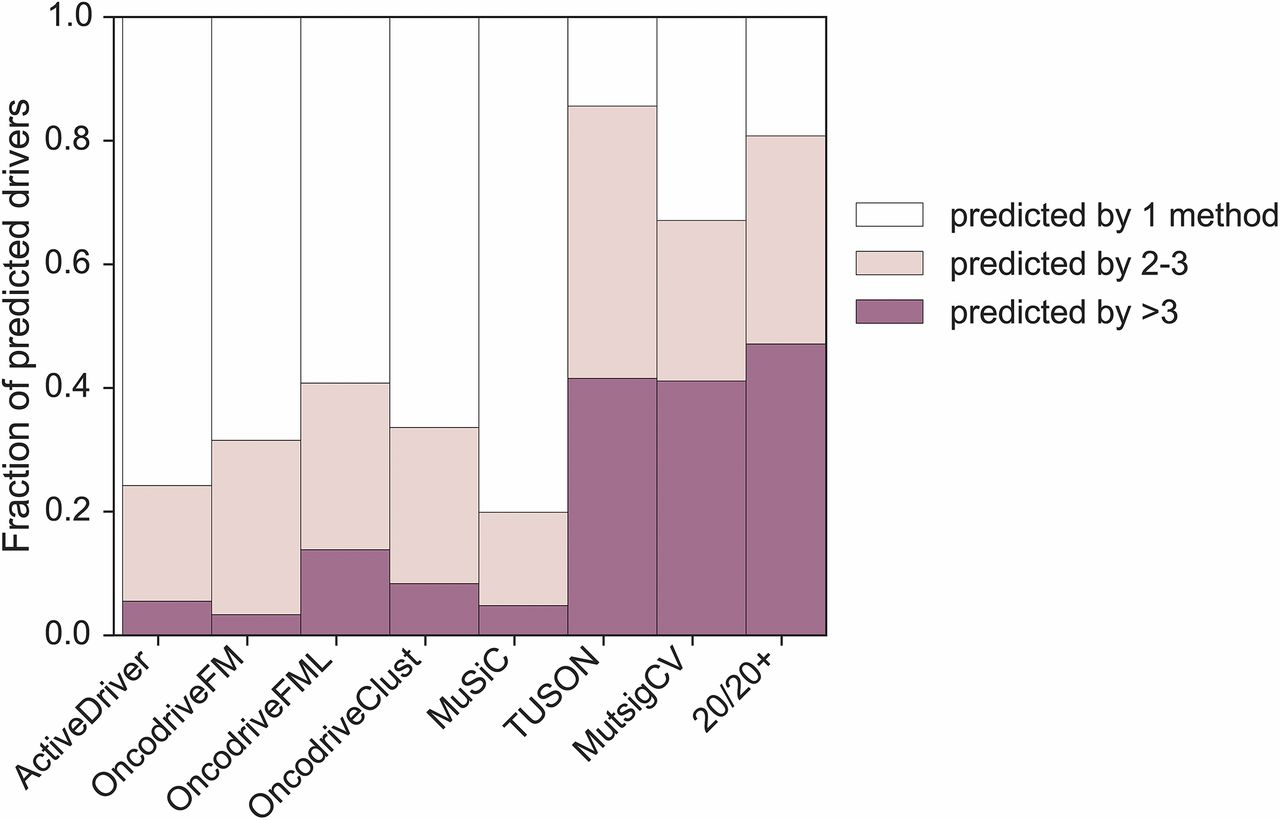
\includegraphics[width=0.9\linewidth]{figures/chapter4/method_overlap.jpg}
  \caption[Consensus among driver gene methods]{Fraction of predicted driver genes for each method by consensus among methods. Fraction of predicted drivers unique to each method, predicted by two to three methods or predicted by more than three methods are shown. A predicted driver gene is defined by Benjamini-Hochberg adjusted P value ($q \leq 0.1$)}
  \label{fig:benchmark_method_overlap}
\end{figure}

\section{Observed vs. Expected P Values}

Given the lack of agreement among these various methods, I compared P values reported by each method to those expected theoretically. Such comparisons are often used in statistics and can indicate invalid assumptions or inappropriate heuristics. Theoretically, the P value distribution should be approximately uniform after likely driver genes are removed \cite{RN188}. Therefore, I removed all genes predicted to be drivers by at least three methods after Benjamini-Hochberg multiple-testing correction ($q \leq 0.1$) and any remaining genes in the CGC. I assumed that the number of bona fide driver genes not removed by this procedure would be small enough to have minimal impact on the P value distribution. To quantify the differences between the observed P values and those expected from a uniform distribution, I developed a measure named mean absolute log2 fold change (MLFC) (see \autoref{sec:mlfc_justification}). MLFC values near zero represent the smallest discrepancies and the closest agreement between observed and theoretical P values.

One method (20/20+) had an MLFC that was fivefold lower than the seven others (\autoref{fig:benchmark_result}B). I also compared observed and theoretical P values with quantile-quantile plots, which provide a detailed view of P value behavior (\autoref{fig:qq_plot}A). 20/20+ P values had by far the best agreement with theoretical expectation across the entire range of supported values. In the critical range typically used to assess statistical significance ($P \leq 0.05$), OncodriveClust, OncodriveFM, OncodriveFML, ActiveDriver, and MuSiC substantially underestimated P values, whereas MutsigCV substantially overestimated them (\autoref{fig:qq_plot}B). For methods that combine multiple P values for each gene, failure to model correlation between P values may be responsible for this underestimation. The null P value distributions at the other end of the distribution (0.2-1.0) should also be uniform and in this case independent of the actual number of true driver genes.

\begin{figure}
  \centering
  \makeatletter
  \let\@currsize\normalsize
  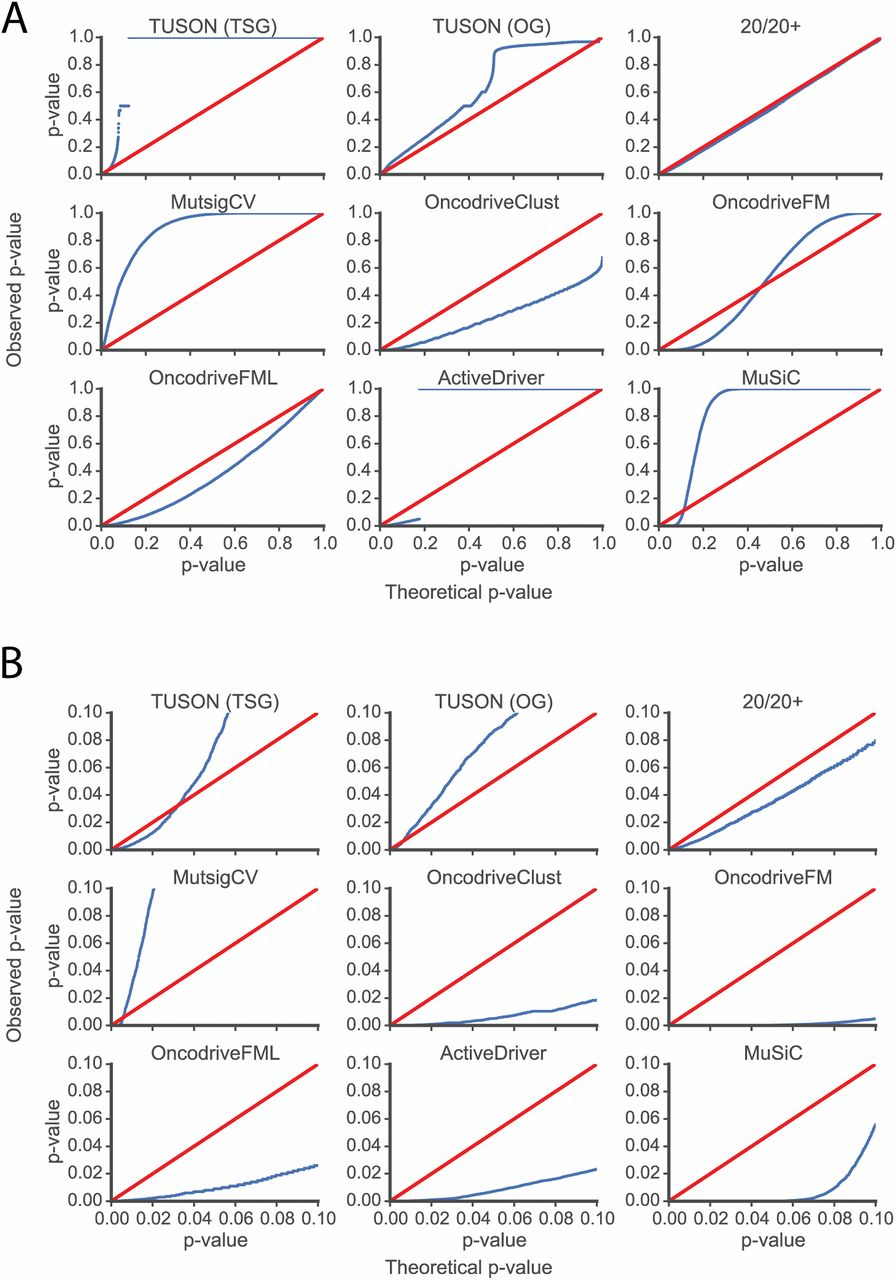
\includegraphics[width=0.9\linewidth]{figures/chapter4/qq_plots.jpg}
  \caption[Quantile-quantile plots comparing observed and theoretical P values]{Quantile-quantile plots comparing observed and theoretical P values for the tested methods. (A) Full P value range from 0 to 1. (B) Blowup of P values from 0 to 0.1. Observed P values for the methods (blue) are compared with those expected from a uniform distribution (red). Genes predicted as drivers by at least three methods were removed along with genes in the CGC. TUSON OG and TSG P values are shown separately.}
  \label{fig:qq_plot}
\end{figure}

\subsection{MLFC and mathematical justification}
\label{sec:mlfc_justification}

The MLFC is a metric of discrepancy between an observed P value distribution reported by a method and a theoretical uniform null distribution. I define MLFC as follows,

\begin{equation}
MLFC=1/n\sum_{i=1}^{n}{\left|\log_2{\frac{P(i)}{i/n}}\right|}
\end{equation}

where P(i) = i'th smallest P value, n is the total number of genes after excluding likely driver genes, and i/n is the corresponding expected P value from a uniform distribution. Values of MLFC near zero indicate smaller discrepancies, and therefore better statistical modeling of the passenger gene null distribution. The absolute value was included to prevent p-value distributions which show evidence of over-dispersion from effectively canceling out over-estimation of p-values with under-estimation in other p-values (see OncodriveFM, \autoref{fig:qq_plot}A).

All methods evaluated in the benchmark here used the Benjamini-Hochberg (BH) method \cite{RN94} to control the false discovery rate. The BH procedure rejects hypotheses by selecting the largest index g such that,

\begin{equation}
\frac{P(i)}{i/n} \leq q^*
\end{equation}
where $q^*$ is the desired false discovery rate control, and then rejecting all hypotheses $H(i)$ from index $i=1,..,g$. The critical part of the MLFC equation is the ratio of observed p-value to expected, which is intentionally the same statistic used in the Benjamini-Hochberg method. There are alternative approaches for testing whether a probability distribution differ from theoretical expectations, such as the Kolmogorov-Smirnov (KS) test \cite{RN100}. The KS test evaluates the significance of the maximum absolute differences between cumulative distribution functions. However, given the large number of hypothesis tests, even small absolute differences in the cumulative distribution at small p-values may result in many false positives. Moreover, I reasoned that in contrast to MLFC, the KS statistic does not directly relate to the BH procedure and disproportionately focuses on discrepancies at large p-values, which are of less practical interest.

\section{Number of Predicted Driver Genes}

The number of predicted driver genes ($q \leq 0.1$) ranged from 158 (MutsigCV) to 2,600 (OncodriveFM) (\autoref{fig:benchmark_result}C). There were two obvious categories of methods with respect to predicted driver genes: MutSigCV, 20/20+, and TUSON predicted 158-243 genes, whereas the remaining had over 400 driver genes.

\section{Driver Gene Prediction Consistency}

Statistical methods suffer from both systematic and random prediction errors. When no gold standard is available, it is difficult to estimate systematic error, but possible to estimate random error by measuring the variability of predictions. I tested the eight methods on 10 repetitions of a random two-way split of the all samples in our dataset, while maintaining the proportion of samples in each cancer type. An ideal method would produce the same list of driver genes, ranked by P value, for each half of the split. For a fair comparison, I considered that methods predicting many drivers would be less likely to have consistent rankings than those predicting only a few. Thus, I developed a measure named TopDrop consistency (TDC) (see \autoref{sec:tdc_limitations}) that examines the overlap between genes ranked at a defined depth (e.g., the top 100 genes) for each half of the random split. Examining TDC at a depth of 100 genes showed MuSiC, 20/20+, and TUSON to be the three with the highest consistency (\autoref{fig:benchmark_result}D). Most methods decreased in consistency when the gene depth was varied between 20 and 300, but the ordering of the TDC scores among the eight methods remained relatively stable.

\subsection{TopDrop consistency and limitations}
\label{sec:tdc_limitations}

Consistency assesses stability in gene ranking. Each method was applied to 10 repeated random splits, consisting of two disjoint halves of the full data. For pancancer assessment, the proportion of samples from each cancer type was maintained in each half. Disjoint halves were scored separately by each method, and genes were ranked from low to high P values. For a fair comparison between methods, I considered a specific depth of top-ranked genes, rather than a fixed q value threshold. This is because consistency becomes harder to achieve as the number of top-ranked genes gets larger. For example, a method that predicts 100 significant genes at $q \leq 0.1$ has an advantage in consistency over a method that predicts 1,000 significant genes at that threshold. I define $TopDrop consistency=|I_d |/d$, where $d$ is the designated depth of interest for the ranked gene list and $I_d$ is the TopDrop intersection, $I_d=A^{(1:d)} \cap B^{(1:2d)}$, defined as the intersection between predictions from the two random halves "A" and "B" such that the top d genes in "A" do not fall past twice the designated depth (2d) in "B."

I expect that all methods will lose statistical power and have greater random sampling error when they are predicting on a dataset that has been split in half. Therefore, I chose to allow genes to fall twice as far down the list in the "B" half of the split, to better distinguish random effects and methods with intrinsically low consistency.

A substantial limitation is TopDrop only evaluates consistency with independent identically distributed samples from the same data set. A better alternative would be to evaluate cross-study consistency \cite{RN157}, as there may be multiple reasons why findings in one study would not generalize to another. However, from a practical perspective, I can only use data currently available to evaluate performance.

\section{Overall Performance}

In \autoref{tab:overall_performance}, I summarize the performance of each method according to the criteria described above on the pancancer mutation data. The overall protocol is shown as a flowchart in \autoref{fig:flow_chart}. I assume that a preferable method would predict a higher fraction of driver genes that overlap with the CGC, that overlap with at least one other method, that have the least deviation from expected null P values, and that have the highest consistency. Each method is accordingly ranked by these four criteria and the average rank is shown. The top ranked methods are 20/20+, TUSON, OncodriveFML, and MutsigCV.

\makeatletter
\let\@currsize\normalsize
\ssp
\begin{sidewaystable}
\begin{tabular}{p{3cm} p{3cm} p{2.25cm} p{2.25cm} p{2.25cm} p{2.25cm} p{2.25cm}}
\toprule
  Method & No. significant genes &  CGC rank &  Consensus rank &  Pvalue rank &  Consistency rank &  Average rank \\
\midrule
  2020+ &  208 &  1 &  2 &  1 &  2 &  1.50 \\
  TUSON &  243 &  2 &  1 &  2 &  3 &  2.00 \\
  OncodriveFML &  679 &  4 &  4 &  3 &  4 &  3.75 \\
  MutsigCV &  158 &  3 &  3 &  4 &  6 &  4.00 \\
  OncodriveClust &  586 &  5 &  5 &  6 &  7 &  5.75 \\
  MuSiC &  1,975 &  7 &  8 &  8 &  1 &  6.00 \\
  ActiveDriver &  417 &  6 &  7 &  5 &  8 &  6.50 \\
  OncodriveFM &  2,600 &  8 &  6 &  7 &  5 &  6.50 \\ 
\bottomrule
\end{tabular}
\caption[Overall performance identifying cancer driver genes]{Performance of eight evaluated cancer driver gene prediction methods on the pancancer dataset of small somatic mutations}
\label{tab:overall_performance}
\end{sidewaystable}
\dsp

\begin{figure}
  \centering
  \makeatletter
  \let\@currsize\normalsize
  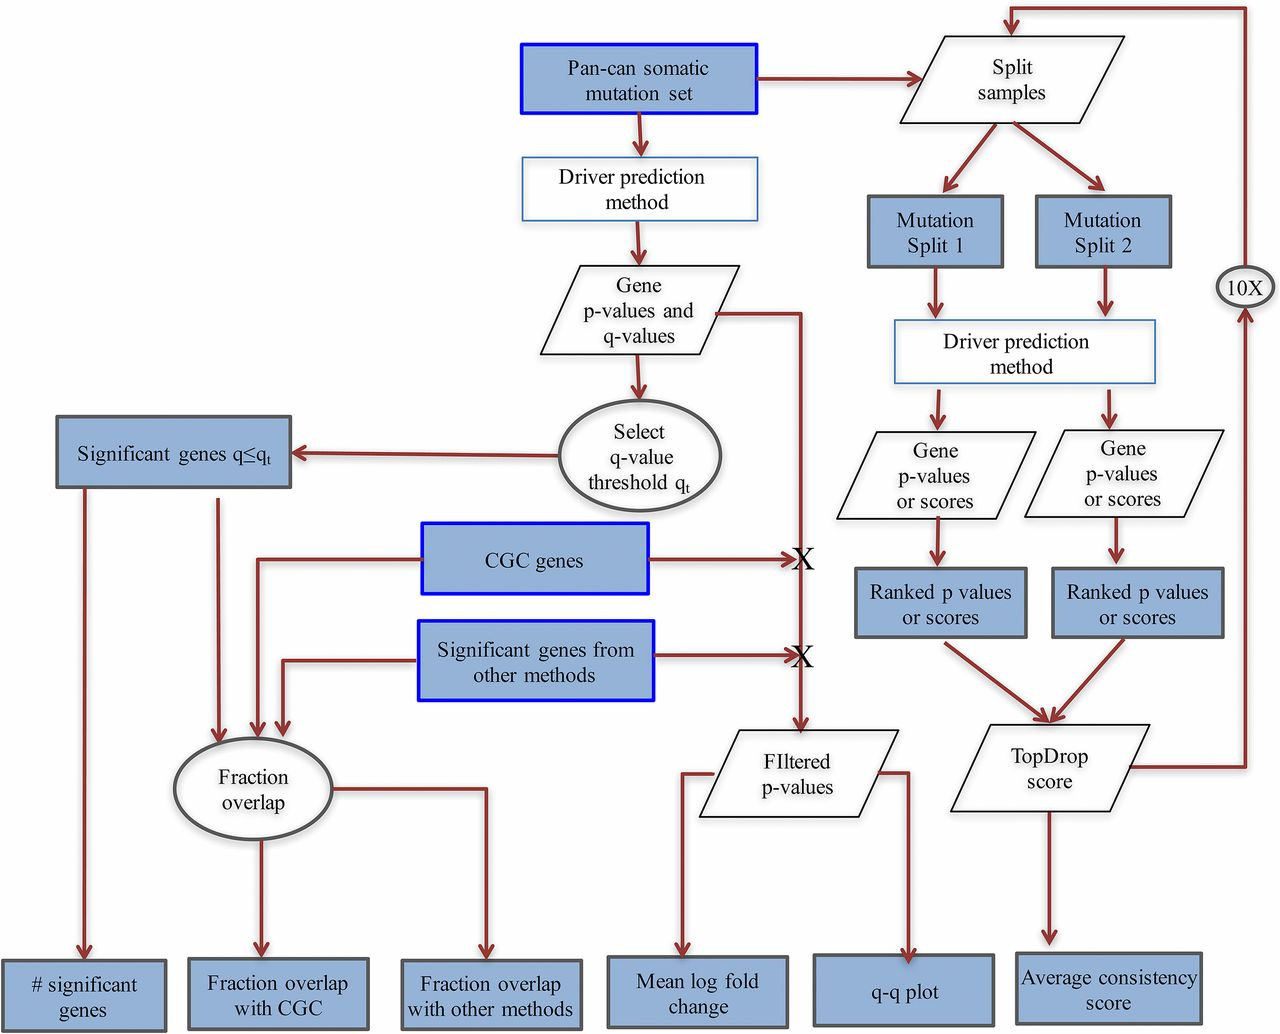
\includegraphics[width=0.9\linewidth]{figures/chapter4/flow_chart.jpg}
  \caption[Flowchart of driver gene evaluation protocol.]{Flowchart of evaluation protocol. Overview of how a driver gene prediction method of interest can be evaluated. The input to the method is the pancan somatic mutation set provided in this work \cite{RN70}. The initial output from the method to be evaluated is a list of predicted driver genes with associated P values and q values. A list of significant driver genes is produced by selecting a q value threshold. To compute fraction overlap of genes predicted as significant with Cancer Gene Census (CGC) and with the eight methods evaluated here, a freeze of CGC and predictions from the eight methods are provided. These gene lists are also used to subtract out putative driver genes and yield a list of filtered P values. Method consistency is estimated by 10 iterations of splitting the pancan somatic mutation set, outputting gene P values and scores for both halves, and applying the TopDrop metric. Jupyter notebooks for computing MLFC and qq plots from the filtered P value list, and the average TDC score are available at github.}
  \label{fig:flow_chart}
\end{figure}

\section{Conclusion}

A major goal of the huge public investment in large-scale cancer sequencing has been to find driver genes. Robust computational prediction of drivers from small numbers of somatic variants is critical to this mission, and it is essential that the best methods for this purpose be identified. Although many such methods have been proposed (see review \cite{RN49}), it has been difficult to evaluate them because there is no gold standard to use as a benchmark. Here, I developed an evaluation framework for driver gene prediction methods that does not require a gold standard. The framework includes a large set of small somatic mutations from a wide range of cancer types and five evaluation metrics. It can be used to systematically evaluate new prediction methods and compare them to existing methods. The results would be more informative to users of these methods than current ad hoc approaches.

To apply the framework to a new method (\autoref{fig:flow_chart}), a ranked list of predicted driver genes can be generated from the pancancer mutation dataset, including a P value and a Benjamini-Hochberg corrected q value for each gene. The choice of a threshold $q \leq 0.1$ to define driver genes worked well in our evaluations but can be adjusted if so desired. The same threshold should be used for fair comparison of different methods. If a driver prediction tool does not produce P values, a raw score threshold that represents the desired false-discovery rate could be selected.

The MLFC also has substantial implications for the accuracy of driver gene prediction methods. The relatively high MLFC of several methods brings into question the validity of the assumptions or analytic methods used in their construction. I believe that the most likely problem is with the assumptions rather than the analytic methods, which all appear to be well thought-out. In addition, the most likely problem with the assumptions is that there is unexplained variability in the background mutation rates (see \autoref{chap:ch2}). This variability may be tumor type specific or even patient or tumor specific. If P values are underestimated in the range of low p-values, too many genes will be called as drivers. In fact, the methods that underestimate P values predict the largest number of drivers and have the highest fraction of uniquely predicted drivers.


